\documentclass[a4paper, 12pt, twocolumn]{article}
\usepackage[T1]{fontenc}
\usepackage{graphicx} % Required for inserting 
\usepackage{lipsum} % for mock text
\usepackage{float}
\usepackage{tikz}
\usepackage[colorlinks=true, urlcolor=blue, linkcolor=red]{hyperref}

\begin{document}

\title{Calculating the Speed of Sound in a Tube}
\author{Parker Wise$^{1}$, Aidan Novo$^{1}$\\$^{1}$University of Kansas}
\date{February 2024}

\twocolumn[
\begin{@twocolumnfalse}
  \maketitle
  \begin{abstract}
The speed of sound is the velocity that a wave propagates at in a gas. The speed of sound for the Earth's atmosphere should be roughly the same everywhere. The speed of sound has been measured both experimentally and calculated theoretically. There is a difference of about 5 m/s between the accepted theoretical value and Derham's experimental value. Through using precise equipment and an isolated environment the speed of sound was calculated within a m/s as 342.6 m/s. 	
  \end{abstract}
\end{@twocolumnfalse}
]
\section{Introduction}
\begin{figure*}[h]
	\centering
	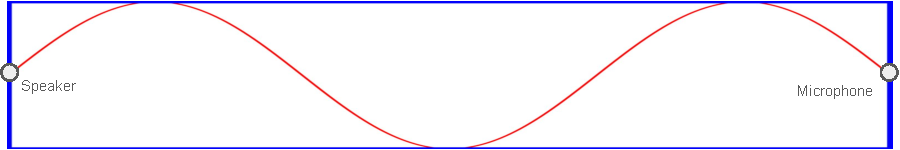
\includegraphics[scale=1]{box.pdf}
	\caption{The apparatus used to obtain the speed of sound. A speaker was hooked up to a signal generator and produced a frequency sweep from 800 Hz to 10 kHz. A microphone at the other end of tube was hooked up to an oscilloscope and the response was recorded.}
	\label{fig:box}
\end{figure*}
Issac Newton originally calculated the speed of sound theoretically as 298 m/s [1]. Pierre-Simon Laplace later corrected this by assuming that the transfer of sound is an adiabatic process [2]. He calculated the speed of sound as 343 m/s. William Derham calculated the speed of sound experimentally by observing the flash of a gun shot as 348 m/s [3]. In the same experimental setup as this experiment, Wellman calculated a speed of 376 m/s [4]. 
\section{Methods}
\begin{figure*}[h]
	\centering
	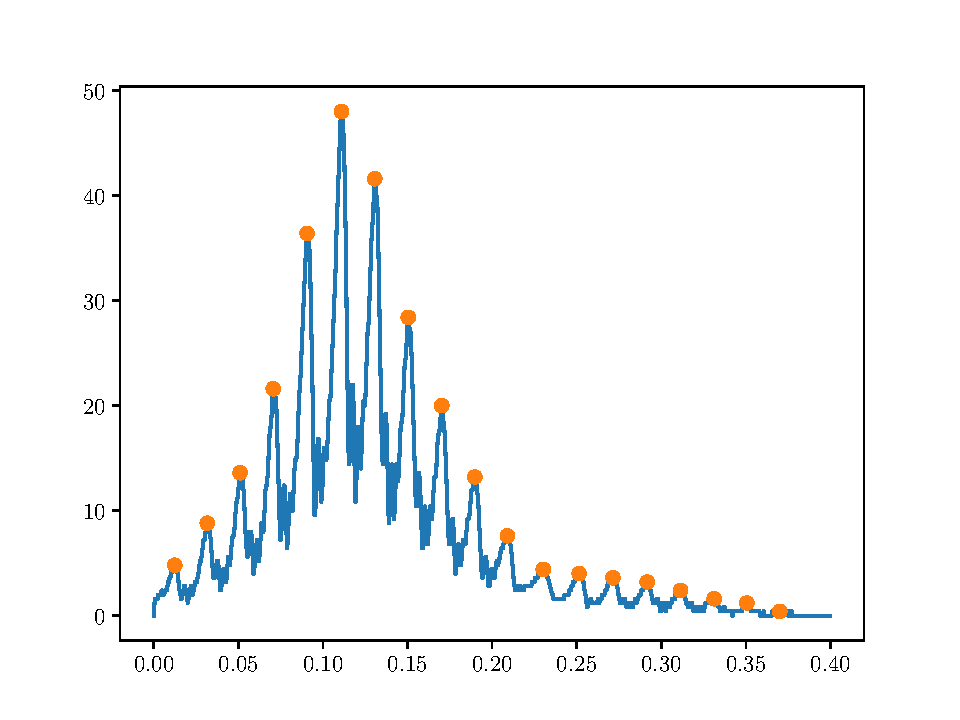
\includegraphics[scale=0.75]{../peaks.pdf}
	\caption{In blue is a plot of the response from the microphone at varying frequencies. Orange dots are located at the resonant frequencies at each local maximum. }
	\label{fig:spectra}
\end{figure*}
The resonant frequencies of a tube can be calculated theoretically based off of its length. The speed of any wave propagates at is described by its wavelength and its frequency.
\begin{equation}
c=\lambda\nu
\end{equation}
The resonant frequencies of a tube are the frequencies in which the wavelength is a standing wave. For any specified distance there are an infinite amount of resonant frequencies with the following wavelengths.
\begin{equation}
\lambda=\frac{2L}{n}
\end{equation}
where L is the length of the tube and n is the index. Putting these two equations together results in a relationship between the speed of sound, the length of the tube, and the resonance's index. 
\begin{equation}
\nu=\frac{2CL}{n}
\end{equation}
If n, L and $\nu$ are known then the speed of sound can be calculated. This equation can also be viewed as a linear realtionship between $\nu$ and n with $\frac{c}{2L}$  being the slope. Simply multiplying by 2L gives us c. 
In order to find this relationship between $\nu$ and n, the apparatus shown in Figure \ref{fig:box} was used. This apparatus has a speaker playing a frequency sweep of sinusoidal waves at one end and a microphone at at the other. At resonant frequenceis the wave will be amplified and the microphone picks that up. Looking at the response of the microphone from each frequencies shows a peak at each resonance. Taking the first identifiable resonant frequency and considering it n=0, and then plotting each consecutive resonance as n+1 on a plot against the frequency will result in the relationship needed to calculate the speed of sound. The speed of sound was then found as $2L$ times the slope of the line that was fit to this data. This was done for several lengths of tube in order to cross check the data. 
In addition to looking at the resonances of a tube, the resonances of a sphere were also investigated. This was done by taking a sphere with two seperate hemispheres, one with a microphone and one with a speaker. The two hemispheres were rotated at 10 degree intervals from 0 degrees to 180 degrees with the same frequency sweep as the tube.  
\clearpage
\section{Results}
\begin{figure*}[ht!]
	\centering
	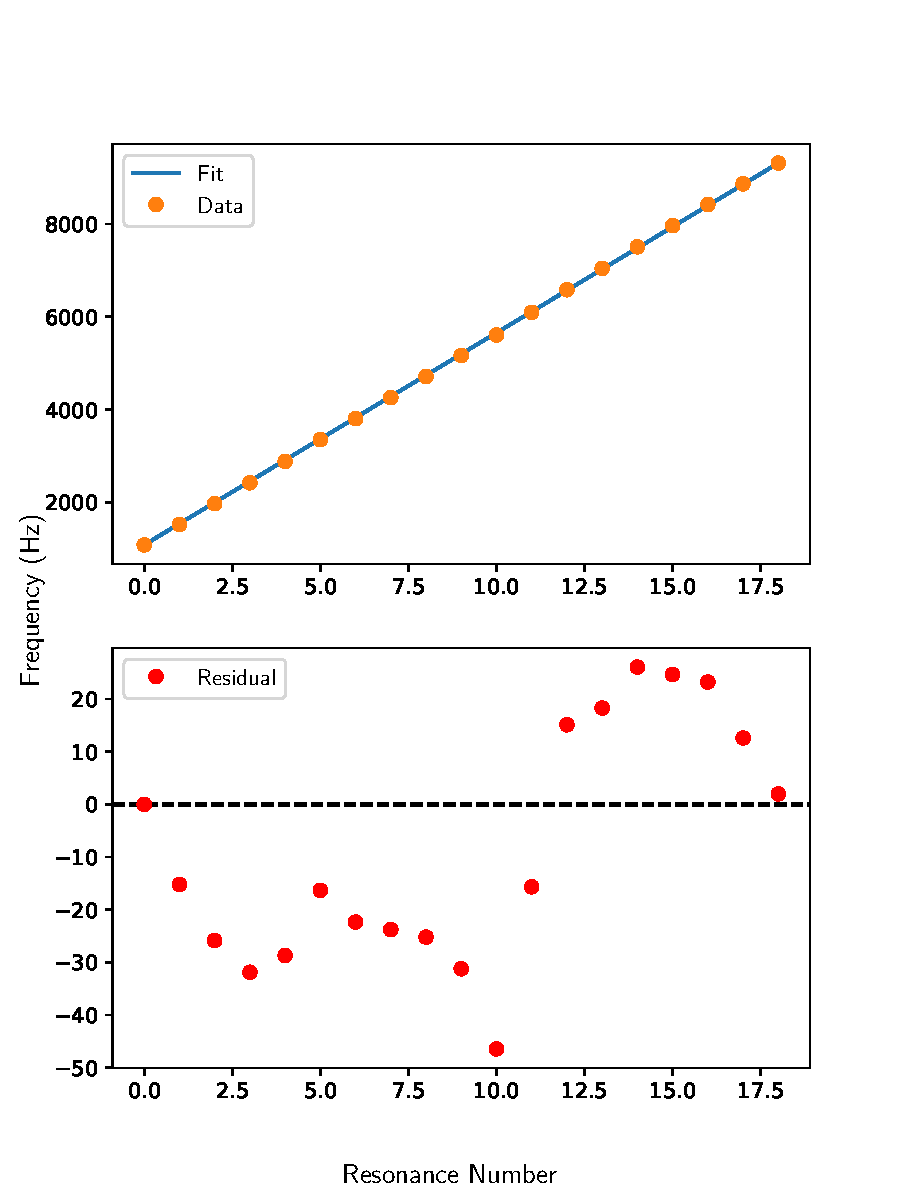
\includegraphics[scale=0.75]{../fitting.pdf}
	\caption{(Top) Each resonant frequencies and their relative index are plotted in orange. A fit was made to this data, represented in blue. (Bottom) the residuals between the fit and the data are shown in red.}
	\label{fig:fit}
\end{figure*}
\begin{figure*}[t!]
	\centering
	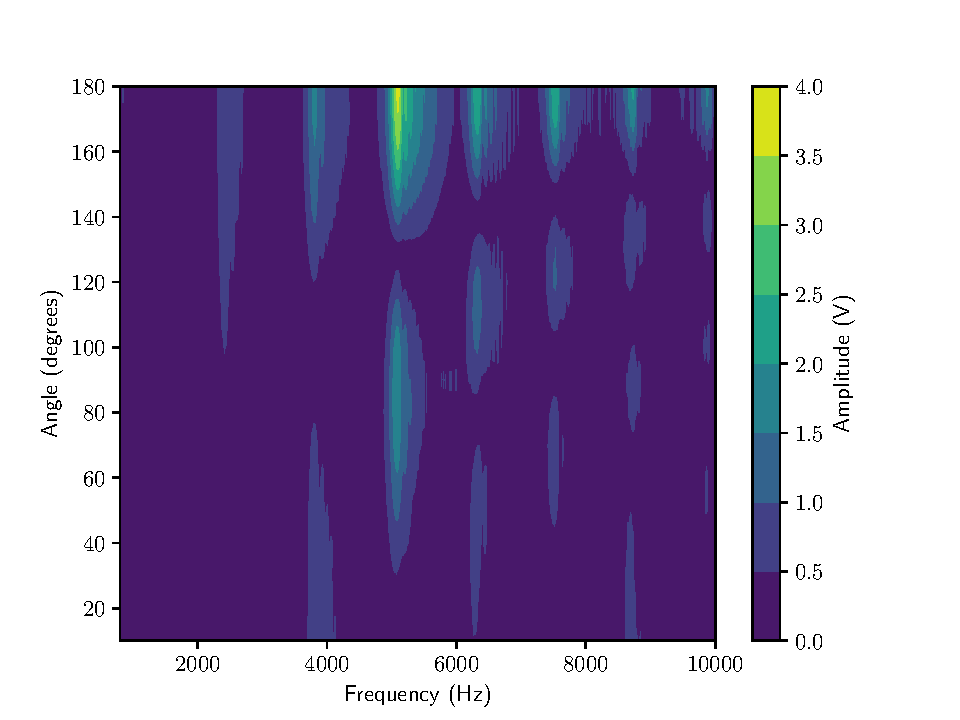
\includegraphics[scale=1]{../Rotation.pdf}
	\caption{A contour map of the response from a frequency sweep done within a sphere with varying angles between the microphone and the speaker.}
	\label{fig:sphere}
\end{figure*}
Figure \ref{fig:spectra} shows the response from the microphone with a tube of 37.5 cm from 800 Hz to 10 kHz. Each peak represents a resonant frequency. Each specific line has a Lorentzian curve. Figure \ref{fig:fit} shows the linear relationship between index number and frequency as predicted by theory. A line was fit to the data and the speed of sound was derived from the slope of the line as discussed in methods. The speed of sound was calculated to be 342.6 m/s $\pm$ 0.4 m/s. The residuals on the fit in Figure \ref{fig:fit} show a slight positive correlation. Considering the small range in residuals compared to the frequency range of the fit, the residuals still point to a good fit of the data. One posibility for this correlation could be the fact that the microphones response is not flat across all frequencies. Calculations were made from multiple lengths. The 37.5 cm tube gave a fit with smallest residuals. A tube of length 30 cm resulted in a speed of sound of 403.92 m/s $\pm$ 3.87 m/s. A tube of length 22.5 resulted in a speed of sound of 502.44 m/s $\pm$ 10.96 m/s.
\section{Conclusion}
The model used in this paper fit to the data with relatively low residuals. This indicates that the theory is likely correct. A connection can be drawn between sound waves and the wave function. The wave function of a particle in a 1D infinite square is a standing wave. In this way, the resonant frequencies of a tube serve as an analog to the different energy states of the particle in a 1D infinite square well. The spherical case applies here too. Instead of a 1D infinite square well, the sphere serves as an analog of the wave functions of the hydrogen atom. The value of the speed of sound derived in this experiment came out to be 343.2 m/s which agrees with the Laplace corrected speed of sound. Wellman got a value of 376 m/s using the same set up. Derham got a speed of 348 m/s. The precise measurements of this experiment affirm the theoretical values derived by Laplace's corrected model of Newton's calculated speed of sound, reaffirming that model. This experiment also serves as an analog to the wave nature of particles viewed through quantum mechanics.
\section*{References}
[1] Issac Newton. Philosophiæ Naturalis Principia Mathematica, 1687.
\par\noindent
[2] Pierre-Simon Laplace. Sur la vitesse du son dans l'air et dans l'eau, 1816.
\par\noindent
[3] William Derham. Experimenta observationes de soni motu, aliisque ad id attinentibus, facta à Reverendo D. W. Derham Ecclesia Upminsteriensis Rectore, & Societatis Regalis Londinensis Socio, 1708. 
\par\noindent
[4] Wellman et al. Measurements of Sound Waves and
Comparisons to Quantum Mechanics, 2024.
\end{document}




